\subsection{Results}
The data from the UMBmark test were used to plot three robot paths.
The points at which the robot stopped to turn were marked on the floor,
and were used as reference points.
The laser range scanner and odometry readings were sent to a PC,
and were processed using the aforementioned algorithms.
A problem occured in the test: some laser range scanner readings were lost,
possibly due to partial incompatibility between the PC's OS and the laser range scanner library used.

However, the line-based localisation algorithm was able to match the features correctly for several
rounds, and the results have been plotted in figure \ref{fig:comparisonOfEncoderVSScanner}.

\begin{figure}[H]
\centering
\makebox[\textwidth][c]{
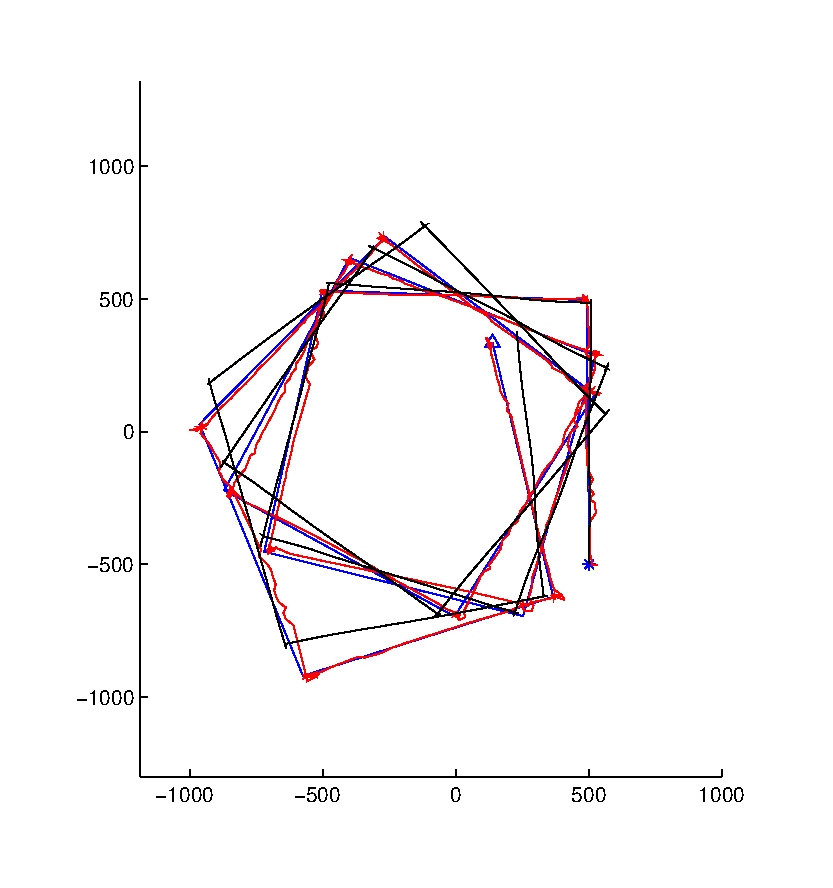
\includegraphics[width = 15cm,trim= 1cm 1cm 1cm 1cm ,clip=true]{graphics/comparison_encoderVSscanner}}
\caption[Comparison of the two localization methods.]{Comparison of the two localization methods.
The blue line connects the reference points where the robot paused to turn,
$*$ is the starting position and $\Delta$ is the ending position.
The red line represents the 2D laser range scanner localisation and the black line represents the odometry readings.}
\label{fig:comparisonOfEncoderVSScanner}
\end{figure}

It is easily seen that the line-based localisation algorithm is better than odometry alone.
The line-based localisation seems to move in distored lines, and this indicates the actual movement
better than the reference lines; The reference lines are just straight lines drawn between the reference points.

\todo[inline,author=Mikael]{Vi mangler resultater for orientering :-)}

The results were expected, as the odometry method accumulates error over time, and the line-based method does not.